\documentclass[12pt,letterpaper]{article}
\usepackage[utf8]{inputenc}
\usepackage{amsmath}
\usepackage{amsthm}
\usepackage{amsfonts}
\usepackage{amssymb}
\usepackage{pgffor}
\usepackage{fullpage}
\usepackage{xcolor}
\usepackage{graphicx}
\usepackage{paratype}
\usepackage{eulervm}
\usepackage{microtype}
\usepackage{tikz}
\usepackage{booktabs}
\usepackage[color=red!5]{todonotes}
\usepackage{url}

\usepackage{minted}
\setminted{bgcolor=gray!10}

\DeclareMathOperator{\SUM}{SUM}
\DeclareMathOperator{\MOD}{MOD}
\DeclareMathOperator{\size}{size}
\DeclareMathOperator{\gates}{gates}

\tikzstyle{input}=[draw=none, inner sep=.2mm]
\tikzstyle{gate}=[draw, circle, inner sep=.2mm, minimum size=5mm]
\tikzstyle{l}=[draw=none, rectangle, fill=white, inner sep=.4mm]


\newenvironment{mypic}{\begin{center}\begin{tikzpicture}}{\end{tikzpicture}\end{center}}



\begin{document}
\sloppy

\title{SAT-based Circuit Local Improvement}
\author{Alexander~S. Kulikov \and Nikita Slezkin}
\maketitle

\begin{abstract}
Finding exact circuit size 
is a~notorious optimization
problem in practice. Whereas modern computers 
and optimization techniques allow to~find a~circuit 
of~size seven in~blink of an~eye, it~may take more 
than a~week to~search for a~circuit of~size thirteen.
One of the reasons of this behavior is that the search 
space is~enormous: the number of circuits of size~$s$ 
is~$s^{\Theta(s)}$, the number of Boolean functions on~$n$ variables is~$2^{2^n}$.

In~this paper, we~explore the following natural
heuristic idea for decreasing the size of
a~given circuit: go through all its subcircuits
of moderate size and check whether 
any of them can be improved by reducing to~SAT. 
This may be viewed
as a~local search approach: we search for a~smaller
circuit in a~ball around a~given circuit.
We~report the results of experiments with various symmetric functions. 
\end{abstract}

\tableofcontents

\clearpage


%\end{document}

\section{Boolean Circuits}
A~Boolean \emph{straight line program} 
%or a~\emph{circuit} 
of size~$r$ for input variables $(x_1, \dotsc, x_n)$ 
is a~sequence of~$r$~instructions where each 
instruction $g \gets h \circ k$ 
applies a~binary Boolean operation~$\circ$ to 
two operands $h,k$ each of which is either an input bit 
or the result of a~previous instruction. 
If $m$~instructions are designated as outputs,
the straight line program computes a~function 
$\{0,1\}^n \to \{0,1\}^m$ in a~natural way. For 
a~Boolean function $f \colon \{0,1\}^n \to \{0,1\}^m$,
by $\size(f)$ we denote the minimum size of 
a~straight line program
computing~$f$. A~Boolean \emph{circuit} 
shows a~flow graph of a~program.

Figure~\ref{figure:sum23} gives an~example for
the 
$\SUM_n \colon \{0,1\}^n \to \{0,1\}^l$ function 
that computes the binary representation of~the sum of~$n$~bits:
\[\SUM_n(x_1, \dotsc, x_n)=(w_0, w_1, \dotsc, w_{l-1})\colon \sum_{i=1}^{n}x_i=\sum_{i=0}^{l-1}2^iw_i \text{, \, where } l=\lceil \log_2(n+1)\rceil \, .\]
This function transforms $n$~bits 
of weight~0 into $l$~bits 
of~weights $(0,1,\dotsc,l-1)$.
%
\begin{figure}[ht]
\begin{minipage}{.28\textwidth}
\begin{minted}{python}
def sum2(x1, x2):
    w0 = x1 ^ x2
    w1 = x1 * x2
    return w0, w1
\end{minted}
\end{minipage}
\begin{minipage}{.18\textwidth}
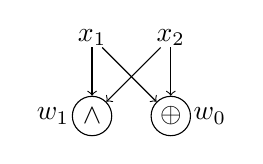
\begin{tikzpicture}[label distance=-.9mm]
\foreach \n/\x/\y in {1/0/1, 2/1/1}
  \node[input] (x\n) at (\x, \y) {$x_{\n}$};
\node[gate, label=left:$w_1$] (g1) at (0,0) {$\land$};
\node[gate, label=right:$w_0$] (g2) at (1,0) {$\oplus$};
\foreach \f/\t in {x1/g1, x1/g2, x2/g1, x2/g2}
  \draw[->] (\f) -- (\t);
\end{tikzpicture}
\end{minipage}
\begin{minipage}{.33\textwidth}
\begin{minted}{python}
def sum3(x1, x2, x3):
    a = x1 ^ x2
    b = x2 ^ x3
    c = a | b
    w0 = a ^ x3
    w1 = c ^ w0
    return w0, w1
\end{minted}
\end{minipage}
\begin{minipage}{.18\textwidth}
~
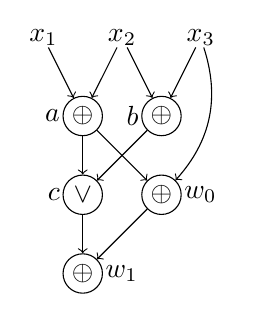
\begin{tikzpicture}[label distance=-.9mm]
\foreach \n/\x/\y in {1/0/3, 2/1/3, 3/2/3}
  \node[input] (x\n) at (\x, \y) {$x_{\n}$};
\node[gate,label=left:$a$] (g1) at (0.5,2) {$\oplus$};
\node[gate,label=left:$b$] (g2) at (1.5,2) {$\oplus$};
\node[gate,label=left:$c$] (g3) at (0.5,1) {$\lor$};
\node[gate, label=right:$w_0$] (g4) at (1.5,1) {$\oplus$};
\node[gate, label=right:$w_1$] (g5) at (0.5,0) {$\oplus$};
\foreach \f/\t in {x1/g1, x2/g1, x2/g2, x3/g2, g1/g3, g2/g3, g1/g4, g3/g5, g4/g5}
  \draw[->] (\f) -- (\t);
\path (x3) edge[bend left,->] (g4);
\end{tikzpicture}
\end{minipage}
\caption{Optimal size straight line programs and circuits for $\SUM_2$ and $\SUM_3$. These two circuits are known as~\emph{half adder} and \emph{full adder}.}
\label{figure:sum23}
\end{figure}
%
The straight line
programs are given 
in~\texttt{Python} programming language.
This makes it particularly easy to verify the correctness of the presented straight line programs.
For example, the program for $\SUM_3$ can be verified
with just three lines of code:
\begin{minted}{python}
from itertools import product


for x1, x2, x3 in product(range(2), repeat=3):
    w0, w1 = sum3(x1, x2, x3)    
    assert x1 + x2 + x3 = w0 + 2 * w1
\end{minted}

\todo[inline]{Nikita, please ensure that this code works}

Determining $\size(f)$ requires
proving lower bounds:
to~show that $\size(f)> \alpha$,
one needs to~prove that \emph{every} circuit
of~size at~most~$\alpha$ does not compute~$f$.
Known lower bounds are far from being satisfactory:
the strongest known lower bound for a~function family
in~NP is~$(3+1/86)n-o(n)$~\cite{}. But even proving
lower bounds for specific functions (rather than function families) is difficult. 
\todo[inline]{tell how Knuth enumerated circuits of four and five variables}
A~natural approach is to~translate a~statement ``there exists a~circuit of size~$11$ computing $\SUM_5$'' into conjunctive normal form formula and feed this formula
to a~SAT-solver. The state-of-the-art SAT-solvers are surprisingly efficient and allow to~handle
various practically important problems (with millions
of~variables) and even help to~resolve some open
problems~\cite{}. Such SAT-based circuit synthesis approach was proposed by~Kojevnikov et al.~\cite{}
and, since then, has been used in various circuit synthesis programs~\cite{}. We demonstrate the limits
of this approach on \emph{counting} functions:
\[\MOD_n^{m,r}=[x_1+\dotsb+x_n \equiv r \bmod m]\]
(here, $[\cdot]$ is the Iverson bracket: $[S]$~is equal to~$1$ if $S$~is true and is equal to~$0$ otherwise).
Using SAT-solvers, Knuth~\cite[solution to exercise~$480$]{Knuth:2015:ACP:2898950}
found $\size(\MOD_n^{3,r})$ for all $3 \le n \le 5$ and all $0 \le r \le 2$. Based on the found numbers, he made the following conjecture:
\begin{equation}\label{conjecture}
\size(\MOD_n^{3,r})=3n-5-[(n+r) \equiv r\bmod 3] \text{ for all $n \ge 3$ and $r$.}
\end{equation}
He was also able to find the circuit size 
for the $n=6,r=0$ case and wrote: ``The case $n=6$ and $r \neq 0$, which lies tantalizingly close to the limits of 
today's solvers, is still unknown.'' 

To~summarize, our current abilities for checking whether there exists a~Boolean circuit of size~$s$ are roughly the following: 
\begin{itemize}
\item for $s \le 6$, this can be done in a~few seconds;
\item for $7 \le s \le 12$, this can (sometimes) 
be~done in a~few days;
\item for $s \ge 13$, this is out of~reach.
\end{itemize}

In this paper, we explore the limits of the following natural idea: given a~circuit, try to~reduce its size by~reducing (using SAT, for example) the size of its subcircuit of size seven. This is a~kind of a~local search approach: we have no possibility to go through the whole space of all circuits, but we can at least
search in a~neighborhood of a~given circuit. 
This allows~us to~work with circuits consisting
of many gates. 

As the results of experiments, we show several circuits
for which the approach described above leads to improved upper bounds. In particular, we support Knuth's conjecture~\eqref{conjecture} by~proving the matching upper bound. We also present improvements for $\size(\SUM_n)$ for various small~$n$. 
Finally, we provide examples of circuits that are
optimal locally, but not globally: our program is not able to find a~(known) smaller circuit since it is 
``too different'' from the original circuit.



\todo[inline]{mention that we are interested in function families}



\section{Program Overview}
The program is~implemented in~\texttt{Python}.
We give a~high-level overview of its main features.
\todo[inline]{create a notebook and state that all the code here can be run in the cloud?}

\subsection{Manipulating Circuits}
This is done through the \mintinline{python}{Circuit}
class. One can load and save circuits as~well~as
print and draw them. A~nicely looking layout of
a~circuit is produced by the \texttt{pygraphviz} module \cite{}. The program also contains some built-in
circuits that can be used as~building blocks.
The following sample code constructs a~circuit
for $\SUM_5$ out of two full adders and 
one half adder. This construction is~shown 
in~Figure~\ref{figure:sumfive}(a). Then, 
the circuit is verified via the  
\mintinline{python}{check_sum_circuit} method. 
Finally, the circuit is drawn. As a~result, one gets
a~picture similar to~the one in~Figure~\ref{figure:sumfive}(b).

\begin{minted}{python}
circuit = Circuit(input_labels=['x1', 'x2', 'x3', 'x4', 'x5'])
x1, x2, x3, x4, x5 = circuit.input_labels
a0, a1 = add_sum3(circuit, [x1, x2, x3])
b0, b1 = add_sum3(circuit, [a0, x4, x5])
w1, w2 = add_sum2(circuit, [a1, b1])
circuit.outputs = [b0, w1, w2]
check_sum_circuit(circuit)
circuit.draw('sum5.png')
\end{minted}

\begin{figure}[ht]
\begin{mypic}
%\draw[help lines] (0,-5) grid (16,6);
\begin{scope}[yshift=-10mm]
\foreach \n in {1,...,5}
  \node[input] (\n) at (\n,6) {$x_{\n}$};
\draw (0.5, 5.5) rectangle (3.5, 4.5); \node at (2, 5) {$\SUM_3$};
\foreach \n in {1, 2, 3}
  \draw[->] (\n) -- (\n, 5.5);
\draw (2.5, 3.5) rectangle (5.5, 2.5); \node at (4, 3) {$\SUM_3$};
\path (3, 4.5) edge[->] node[l] {0} (3, 3.5);
\foreach \n in {4, 5}
  \draw[->] (\n) -- (\n, 3.5);
\draw (1.5, 1.5) rectangle (3.5, 0.5); \node at (2.5, 1) {$\SUM_2$};
\path (2, 4.5) edge[->] node[l] {1} (2, 1.5);
\path (3, 2.5) edge[->] node[l] {1} (3, 1.5);
\node[input] (w2) at (2,-1) {$w_2$};
\node[input] (w1) at (3,-1) {$w_1$};
\node[input] (w0) at (4.5,-1) {$w_0$};
\path (2, 0.5) edge[->] node[l] {1} (w2);
\path (3, 0.5) edge[->] node[l] {0} (w1);
\path (4.5, 2.5) edge[->] node[l] {0} (w0);
\end{scope}

\begin{scope}[label distance=-1mm, xshift=70mm, yshift=20mm]
\foreach \n/\x/\y in {1/0/3, 2/1/3, 3/2/3, 4/2.5/1, 5/3.5/1}
  \node[input] (x\n) at (\x, \y) {$x_{\n}$};
\node[gate,label=left:$g_1$] (g1) at (0.5,2) {$\oplus$};
\node[gate,label=left:$g_2$] (g2) at (1.5,2) {$\oplus$};
\node[gate,label=left:$g_3$] (g3) at (0.5,1) {$\lor$};
\node[gate,label=left:$g_4$] (g4) at (1.5,1) {$\oplus$};
\node[gate,label=left:$g_5$] (g5) at (0.5,0) {$\oplus$};
\node[gate,label=left:$g_6$] (g6) at (2,-1) {$\oplus$};
\node[gate,label=right:$g_7$] (g7) at (3,-1) {$\oplus$};
\node[gate,label=right:$g_8$] (g8) at (2,-2) {$\lor$};
\node[gate, label=right:$w_0$] (g9) at (3,-2) {$\oplus$};
\node[gate, label=right:$g_9$] (g10) at (2,-3) {$\oplus$};
\node[gate, label=right:$w_1$] (g11) at (2,-4) {$\oplus$};
\node[gate, label=left:$w_2$] (g12) at (1,-4) {$\land$};

\foreach \f/\t in {x1/g1, x2/g1, x2/g2, x3/g2, g1/g3, g2/g3, g1/g4, g3/g5, g4/g5, g4/g6, x4/g6, x4/g7, x5/g7, g6/g8, g7/g8, g8/g10, g6/g9, g9/g10, g10/g11, g10/g12}
  \draw[->] (\f) -- (\t);

\path (x3) edge[->,bend left] (g4);
\path (x5) edge[->,bend left=35] (g9);
\path (g5) edge[->,bend right=25] (g11);
\path (g5) edge[->,bend right=15] (g12);

\draw[dashed] (-0.5,-0.25) rectangle (2,2.5);
\draw[dashed] (1.25,-3.25) rectangle (4,-0.5);
\draw[dashed] (0,-3.5) rectangle (3,-4.5);
\end{scope}

\begin{scope}[label distance=-1mm, xshift=120mm, yshift=20mm]
\foreach \n/\x/\y in {1/0/3, 2/1/3, 3/2/3, 4/2.5/1, 5/3.5/1}
  \node[input] (x\n) at (\x, \y) {$x_{\n}$};
\node[gate,label=left:$g_1$] (g1) at (0.5,2) {$\oplus$};
\node[gate,label=left:$g_2$] (g2) at (1.5,2) {$\oplus$};
\node[gate,label=left:$g_3$] (g3) at (0.5,1) {$\lor$};
\node[gate,label=left:$g_4$] (g4) at (1.5,1) {$\oplus$};
\node[gate,label=left:$g_5$] (g5) at (0.5,0) {$\oplus$};
\node[gate,label=left:$g_6$] (g6) at (2,0) {$\oplus$};
\node[gate,label=right:$g_7$] (g7) at (3,0) {$\oplus$};
\node[gate,label=right:$g_8$] (g8) at (2,-1) {$>$};
\node[gate, label=right:$w_0$] (g9) at (3,-1) {$\oplus$};
\node[gate, label=right:$w_1$] (g10) at (2,-2) {$\oplus$};
\node[gate, label=right:$w_2$] (g11) at (1.5,-3) {$>$};

\foreach \f/\t in {x1/g1, x2/g1, x2/g2, x3/g2, g1/g3, g2/g3, g1/g4, g3/g5, g4/g5, x4/g6, g4/g6, x4/g7, x5/g7, g6/g8, g7/g8, g7/g9, g3/g10, g8/g10, g10/g11, g5/g11}
  \draw[->] (\f) -- (\t);

\path (x3) edge[->,bend left] (g4);
\path (g4) edge[->,bend left=20] (g9);
\end{scope}

\foreach \x/\n in {3/a, 9/b, 14/c}
  \node at (\x,-3) {(\n)};
\end{mypic}
\caption{(a)~A~schematic circuit for $\SUM_5$ composed out of two full adders and one half adder. (b)~The corresponding circuit of size~$12$. (c)~An~improved circuit of size~$11$.}
\label{figure:sumfive}
\end{figure}

\subsection{Finding Optimum Circuits}
The method \mintinline{python}{find_circuit}
checks whether there exists a~circuit of the required
size for a~given Boolean function. For example, 
one may discover the full adder as follows.

\todo[inline]{Nikita, Sasha: think about an interface where one only needs to specify a function instead of cooking a~truth table}

\begin{minted}{python}
truth_tables = [[], []]
for x in product(range(2), repeat=3):
    truth_tables[0].append(str((sum(x) >> 0) & 1))
    truth_tables[1].append(str((sum(x) >> 1) & 1))
truth_tables[0] = ''.join(truth_tables[0])
truth_tables[1] = ''.join(truth_tables[1])

circuit = find_circuit(3, None, None, 5, truth_tables)
print(circuit)
\end{minted}

This is~done by~encoding the task as~a~CNF formula
and invoking the PicoSAT solver~\cite{DBLP:journals/jsat/Biere08} (via the \texttt{pycosat} module~\cite{pycosat}). The reduction to~SAT is~described 
in~\cite{DBLP:conf/sat/KojevnikovKY09}. It~is used
in~various programs for circuit synthesis~\cite{reduction, abc}.\todo{more links}

As~mentioned in the introduction, the limits 
of~applicability of~this approach (for finding a~circuit of size~$s$) are roughly the following:
for $s \le 6$, it usually works in less than a~minute;
for $7 \le s \le 12$, it may already take up~to 
several hours or days; for $s \ge 13$, it becomes almost impractical. The running time may vary a~lot
for inputs of the same length. In~particular,
it usually takes much longer to~prove that 
the required circuit does not exist (by~proving that the corresponding formula is~unsatisfiable).

\todo[inline]{various bases}

\subsection{Improving Circuits}
The method \mintinline{python}{improve_circuit}
goes through all subcircuits of a~given size
of a~given circuit and checks whether any 
of~them can be~replaced by a~smaller subcircuit 
(computing the same function) via \mintinline{python}{find_circuit}. For example, applying this method 
to~the circuit from Figure~\ref{figure:sumfive}(b)
gives the circuit from Figure~\ref{figure:sumfive}(c)
in ???~seconds.\todo{Nikita, find this value.} This circuit can~be also found via \mintinline{python}{find_circuit} directly, but it takes ??? seconds.\todo{Nikita, find this value}

\todo[inline]{fix gates, forbid wires}




\section{Experimental Evaluation}

\todo[inline]{mention that we focus on symmetric functions}

\subsection{Sum Function}

\subsection{Modulo-3 Function}
%Here

\subsection{Threshold-2 Function}

\subsection{What Else?..}

\section{Further Directions}

\bibliographystyle{plain}
\bibliography{circuits}

\end{document}



\section{Overview}
Let $l=\lceil \log_2(n+1)\rceil$. The function $\SUM_n \colon \{0,1\}^n \to \{0,1\}^{l}$ computes the binary representation of~the sum of~$n$~bits:
$\SUM_n(x_1, \dotsc, x_n)=(w_0, w_1, \dotsc, w_{l-1})$ such that
\[\sum_{i=1}^{n}x_i=\sum_{i=0}^{l-1}2^iw_i \, .\]
This way, the function transform $n$~bits of weight~0 into $l$~bits 
of~weights $(0,1,\dotsc,l-1)$.

This is~a~fundamental symmetric function. In~particular, for any symmetric predicate~$f \colon \{0,1\}^n \to \{0,1\}$,
\[\size(f) \le \size(\SUM_n)+o(n) \, ,\]
where $\size(\cdot)$ is~the circuit size (in~this text, our default computational model is Boolean circuits over the full binary basis).



\section{Circuit Size of $\SUM_n$}%{Circuit Size for Small Input Sizes}
\subsection{Three Inputs}
The exact circuit size of $\SUM_n$ is known for all~$n$ up to~$n=5$. The table below shows upper bounds for some other values of~$n$:
\begin{center}
\begin{tabular}{lccccccccccc}
\toprule
$n$ & $2$ & $3$ & $4$ & $5$ & $6$ & $7$ & $8$ & $9$ & $10$ & $15$ & $31$\\
\midrule
$\size(\SUM_n)$ & $2$ & $5$ & $9$ & $11$ & $16$ & $19$ & $25$ & $ 27$ & $33$ & $53$ & $125$\\
\bottomrule
\end{tabular}
\end{center}
%
Below, we show optimal circuits for $n=2,3$. They are known as half adder and full adder, respectively.
%
\begin{mypic}
\begin{scope}[yscale=.8]
%\draw[help lines] (0,0) grid (16,6);

\begin{scope}[yshift=2cm]
\foreach \n/\x/\y in {1/0/1, 2/1/1}
  \node[input] (x\n) at (\x, \y) {$x_{\n}$};
\node[gate, label=left:$w_1$] (g1) at (0,0) {$\land$};
\node[gate, label=right:$w_0$] (g2) at (1,0) {$\oplus$};
\foreach \f/\t in {x1/g1, x1/g2, x2/g1, x2/g2}
  \draw[->] (\f) -- (\t);
\end{scope}

\begin{scope}[xshift=4cm]
\foreach \n/\x/\y in {1/0/3, 2/1/3, 3/2/3}
  \node[input] (x\n) at (\x, \y) {$x_{\n}$};
\node[gate] (g1) at (0.5,2) {$\oplus$};
\node[gate] (g2) at (1.5,2) {$\oplus$};
\node[gate] (g3) at (0.5,1) {$\lor$};
\node[gate, label=right:$w_0$] (g4) at (1.5,1) {$\oplus$};
\node[gate, label=right:$w_1$] (g5) at (0.5,0) {$\oplus$};
\foreach \f/\t in {x1/g1, x2/g1, x2/g2, x3/g2, g1/g3, g2/g3, g1/g4, g3/g5, g4/g5}
  \draw[->] (\f) -- (\t);
\path (x3) edge[bend left,->] (g4);
\end{scope}
\end{scope}
\end{mypic}

\subsection{From Three Inputs to~the General Case}
These two basic blocks can already be~used to~compute $\SUM_n$ for any~$n$.
E.g., one can compute $\SUM_5$ by a~circuit of~size~12 as~follows:
%
\begin{mypic}
\begin{scope}[yscale=.7]
%\draw[help lines] (0,-5) grid (16,6);
\foreach \n in {1,...,5}
  \node[input] (\n) at (\n,6) {$x_{\n}$};
\draw (0.5, 5.5) rectangle (3.5, 4.5); \node at (2, 5) {$\SUM_3$};
\foreach \n in {1, 2, 3}
  \draw[->] (\n) -- (\n, 5.5);
\draw (2.5, 3.5) rectangle (5.5, 2.5); \node at (4, 3) {$\SUM_3$};
\path (3, 4.5) edge[->] node[l] {0} (3, 3.5);
\foreach \n in {4, 5}
  \draw[->] (\n) -- (\n, 3.5);
\draw (1.5, 1.5) rectangle (3.5, 0.5); \node at (2.5, 1) {$\SUM_2$};
\path (2, 4.5) edge[->] node[l] {1} (2, 1.5);
\path (3, 2.5) edge[->] node[l] {1} (3, 1.5);
\node[input] (w2) at (2,-1) {$w_2$};
\node[input] (w1) at (3,-1) {$w_1$};
\node[input] (w0) at (4.5,-1) {$w_0$};
\path (2, 0.5) edge[->] node[l] {1} (w2);
\path (3, 0.5) edge[->] node[l] {0} (w1);
\path (4.5, 2.5) edge[->] node[l] {0} (w0);
\end{scope}
\end{mypic}

The same trick shows that $\size(\SUM_n) \le 5n+o(n)$. Indeed, 
the $\SUM_3$ circuit replaces three bits of weight~$i$ by two bits of weight~$i$ and $i+1$. Thus, to~get from $n$~bits of weight~$0$ to $l$~bits of weight $(0,\dotsc, l-1)$, one may 
repeatedly apply $\SUM_3$ to three bits of the same weight. 
An~application of~$\SUM_3$ reduces the number of~bits by~one, hence
the number of such applications is~at~most~$n$. What will remain after this step is at most two bits on each of $l=o(n)$~levels. Pictorially, this looks as~follows.

\begin{mypic}
    %\mydefgrid
    \foreach \n/\t/\x in {{x1/x_1/0.5}, {x2/x_2/1}, {x3/x_3/2}, {x4/x_4/2.5}, {x5/x_5/3.5}, {x6/x_6/4}, {x7/x_7/5}, {x8/x_8/5.5}, {x10/x_n/8.5}}
    {
      \node[] (\n) at (\x,6) {$\t$};
      \draw[->] (\n) -- (\x,5.25);
    }
    \foreach \n/\t/\y in {{y1/w_0/4.75}, {y2/w_1/3}, {y3/w_{l-1}/0.5}}
      \node[] (\n) at (9.5,\y) {$\t$};
    \foreach \l/\r/\x/\y in {{0.25/5.25/1.25/4.25}, {1.75/5.25/2.75/4.25}, {3.25/5.25/4.25/4.25}, {4.75/5.25/5.75/4.25}, {7.75/5.25/8.75/4.25}, {1/3.5/2/2.5}, {4/2.5/5/3.5}, {4/0/5/1}}
      \draw (\l,\r) rectangle (\x,\y);
    \foreach \x/\y in {{0.75/4.75}, {2.25/4.75}, {3.75/4.75}, {5.25/4.75}, {8.25/4.75}, {1.5/3}, {4.5/3}, {4.5/0.5}}
      \node[] at (\x,\y) {\small $\SUM_3$};
    \foreach \x/\y/\l/\r in {{1.25/4.75/1.75/4.75}, {2.75/4.75/3.25/4.75}, {4.25/4.75/4.75/4.75}, {5.75/4.75/6.25/4.75}, {2/3/4/3}, {5/3/7/3}, {0.75/4.25/1.25/3.5}, {2.25/4.25/1.75/3.5}, {3.75/4.25/4.25/3.5}, {5.25/4.25/4.75/3.5}, {5.25/1.75/4.75/1.0}, {3.75/1.75/4.25/1.0}, {7.25/4.75/7.75/4.75}}
      \draw[->] (\x,\y) -- (\l,\r);
    \foreach \x/\y/\t in {{6.75/4.75/\cdots}, {7.74/3/\cdots}, {4.5/2/\cdots}}
      \node[] at (\x,\y) {$\t$};
    \foreach \x/\y/\v in {{8.75/4.75/y1}, {8.25/3/y2}, {5/0.5/y3}}
      \draw[->] (\x,\y) -- (\v);
\end{mypic}

In~general, this gives the following upper bound:
if $\size(\SUM_k) \le r$, then for all~$n$, 
\begin{equation}\label{eq:master}
\size(\SUM_n) \le \frac{rn}{k-\lceil \log_2(k+1) \rceil}+o(n) \, .
\end{equation}

\subsection{Five Inputs and Improved General Case}
It~turns out that 
there exists a~smaller circuit for $\SUM_5$
and that it can be used in two different ways
to~improve the general upper bound! The following circuit of size~11 was found by Knuth. This is how he describes it: ``But $s(5)=12$ is \emph{not} optimum, despite the beauty of~7.1.2-(29)!'' (Here, 7.1.2-(29) refers to~the circuit of size~12.)

\begin{mypic}
\begin{scope}[yscale=.8, label distance=-1mm]
\foreach \n/\x/\y in {1/0/3, 2/1/3, 3/2/3, 4/2.5/1, 5/3.5/1}
  \node[input] (x\n) at (\x, \y) {$x_{\n}$};
\node[gate,label=left:$g_1$] (g1) at (0.5,2) {$\oplus$};
\node[gate,label=left:$g_2$] (g2) at (1.5,2) {$\oplus$};
\node[gate,label=left:$g_3$] (g3) at (0.5,1) {$\lor$};
\node[gate,label=left:$g_4$] (g4) at (1.5,1) {$\oplus$};
\node[gate,label=left:$g_5$] (g5) at (0.5,0) {$\oplus$};
\node[gate,label=left:$g_6$] (g6) at (2,0) {$\oplus$};
\node[gate,label=left:$g_7$] (g7) at (3,0) {$\oplus$};
\node[gate,label=left:$g_8$] (g8) at (2,-1) {$>$};
\node[gate, label=right:$w_0$] (g9) at (3,-1) {$\oplus$};
\node[gate, label=right:$w_1$] (g10) at (2,-2) {$\oplus$};
\node[gate, label=right:$w_2$] (g11) at (1.5,-3) {$>$};

\foreach \f/\t in {x1/g1, x2/g1, x2/g2, x3/g2, g1/g3, g2/g3, g1/g4, g3/g5, g4/g5, x4/g6, g4/g6, x4/g7, x5/g7, g6/g8, g7/g8, g7/g9, g3/g10, g8/g10, g10/g11, g5/g11}
  \draw[->] (\f) -- (\t);

\path (x3) edge[->,bend left] (g4);
\path (g4) edge[->,bend left=20] (g9);

\end{scope}
\end{mypic}
%
Using this circuit, one can build a~circuit of size $5+11+2+1=19$ for $\SUM_7$:
\begin{mypic}
\begin{scope}[yscale=.7]
%\draw[help lines] (0,-5) grid (16,6);
\foreach \n in {1,...,7}
  \node[input] (\n) at (\n,6) {$x_{\n}$};
\draw (0.5, 5.5) rectangle (3.5, 4.5); \node at (2, 5) {$\SUM_3$};
\foreach \n in {1, 2, 3}
  \draw[->] (\n) -- (\n, 5.5);
\draw (2.5, 3.5) rectangle (7.5, 2.5); \node at (5, 3) {$\SUM_5$};
\path (3, 4.5) edge[->] node[l] {0} (3, 3.5);
\foreach \n in {4, 5, 6, 7}
  \draw[->] (\n) -- (\n, 3.5);
\draw (1.5, 1.5) rectangle (3.5, 0.5); \node at (2.5, 1) {$\SUM_2$};
\path (2, 4.5) edge[->] node[l] {1} (2, 1.5);
\path (3, 2.5) edge[->] node[l] {1} (3, 1.5);
\draw (2.5, -0.5) rectangle (4.5, -1.5); \node at (3.5, -1) {XOR};
\path (4, 2.5) edge[->] node[l] {2} (4, -0.5);
\path (3, 0.5) edge[->] node[l] {1} (3, -0.5);

\node[input] (w0) at (6,-3) {$w_0$};
\node[input] (w2) at (3.5,-3) {$w_2$};
\node[input] (w1) at (2,-3) {$w_1$};

\path (6, 2.5) edge[->] node[l] {0} (w0);
\path (2, 0.5) edge[->] node[l] {0} (w1);
\path (3.5, -1.5) edge[->]  (w2);
\end{scope}
\end{mypic}
%
Plugging $\size(\SUM_7) \le 19$ into~\eqref{eq:master}, gives an~upper bound $\size(\SUM_n) \le 4.75n$.

Interestingly, the same $\SUM_5$ circuit can be used to~get a~$4.5n$ upper bound! For this, consider two consecutive $\SUM_3$ circuits.
%
\begin{mypic}
\begin{scope}[scale=.7]
%\draw[help lines] (0,0) grid (10,6);
\draw (1,0) rectangle (3,2); \node at (2,1) {$\SUM_3$};
\draw (5,0) rectangle (7,2); \node at (6,1) {$\SUM_3$};
\foreach \n/\x/\y in {3/0/1, 2/1.5/3, 1/2.5/3, 4/5.5/3, 5/6.5/3}
  \node[input] (\n) at (\x,\y) {$x_{\n}$};
\foreach \n/\t/\x/\y in {a1/a_1/2/-1, b1/b_1/6/-1, b0/b_0/8/1}
  \node[input] (\n) at (\x,\y) {$\t$};
\draw[->] (3)--(1,1);
\draw[->] (2)--(1.5,2);
\draw[->] (1)--(2.5,2);
\draw[->] (4)--(5.5,2);
\draw[->] (5)--(6.5,2);
\draw[->] (3,1)--(5,1);
\draw[->] (7,1)--(b0);
\draw[->] (2,0)--(a1);
\draw[->] (6,0)--(b1);
\end{scope}
\end{mypic}
%
Its specification~is: $x_1+\dotsb+x_5=b_0+2(a_1+b_1)$. Its size 
is~equal to~10.

It~turns out that one can construct a~similar block, called MDFA (for modified double full adder), of size~8:
\begin{mypic}
\begin{scope}[scale=.7]
%\draw[help lines] (0,0) grid (10,6);
\draw (1,0) rectangle (7,2); \node at (4,1) {MDFA};
\foreach \n/\x/\y in {3/0/1, 2/1.5/4, 1/2.5/4, 4/5.5/4, 5/6.5/4}
  \node[input] (\n) at (\x,\y) {$x_{\n}$};
\node[gate] (xor1) at (2.5,3) {$\oplus$};
\node[gate] (xor2) at (6.5,3) {$\oplus$};
\foreach \n/\t/\x/\y in {a1/a_1/2/-1, b1/{a_1 \oplus b_1}/6/-1, b0/b_0/8/1}
  \node[input] (\n) at (\x,\y) {$\t$};
\draw[->] (3)--(1,1);
\draw[->] (2)--(1.5,2);
\draw[->] (1) -- (xor1); \draw[->] (2) -- (xor1);
\draw[->] (xor1) -- (2.5,2);
\draw[->] (4)--(5.5,2);
\draw[->] (5)-- (xor2); \draw[->] (xor2) -- (6.5,2); \draw[->] (4) -- (xor2);
%\draw[->] (3,1)--(5,1);
\draw[->] (7,1)--(b0);
\draw[->] (2,0)--(a1);
\draw[->] (6,0)--(b1);
\end{scope}
\end{mypic}
Using this block, one can compute $\SUM_n$ by a~circuit of size $4.5n$ as~follows:

\begin{mypic}
    \foreach \n/\t/\x in {{x1/x_1/0.5}, {x2/x_2/1}, {x3/x_3/1.5}, {x4/x_4/2}, {x5/x_5/3}, {x6/x_6/3.5}, {x7/x_7/4}, {x8/x_8/4.5}, {x9/x_{n-1}/7.75}, {x10/x_n/8.5}}
      \node[] (\n) at (\x,6.5) {$\t$};
    \foreach \n/\x/\a/\b in {{xor1/1/x1/x2}, {xor2/2/x3/x4}, {xor3/3.5/x5/x6}, {xor4/4.5/x7/x8}, {xor5/8.5/x9/x10}}
    {
      %\mysimplegatetwo{\n}{(\x,5.75)}{$\oplus$}{\a}{\b};  
      \node[gate] (\n) at (\x, 5.75) {$\oplus$};
      \draw[->] (\a) -- (\n);
      \draw[->] (\b) -- (\n);
      \path[draw,->] (\n) -- (\x,5.25);
    }
    \foreach \n/\x in {x1/0.5, x3/1.5, x5/3, x7/4, x9/7.75}
      \path[draw,->] (\n) -- (\x,5.25);
    \foreach \n/\t/\y in {{y1/w_0/4.75}, {y2/w_1/3}, {y3/w_{l-1}/0.5}}
      \node[] (\n) at (9.5,\y) {$\t$};
    \foreach \l/\r/\x/\y in {{0.25/5.25/2.25/4.25}, {0.25+2.5/5.25/2.25+2.5/4.25}, {0.25+6.5/5.25/2.25+6.5/4.25}, {1.5/2.5/3.5/3.5}, {3.5/0/5.5/1}}%, {1.75/5.25/2.75/4.25}, {3.25/5.25/4.25/4.25}, {4.75/5.25/5.75/4.25}, {7.75/5.25/8.75/4.25}, {1/3.5/2/2.5}, {4/2.5/5/3.5}, {4/0/5/1}}
      \draw (\l,\r) rectangle (\x,\y);
    \foreach \x/\y in {{1.25/4.75}, {3.75/4.75}, {7.75/4.75}, {2.5/3}, {4.5/0.5}}
      \node[] at (\x,\y) {MDFA};
    \foreach \xa/\xb in {0.75/1.75, 1.25/2.25, 3.75/2.75, 4.25/3.25}
      \draw[->] (\xa,4.25) -- (\xb,3.5);
    \foreach \x/\y/\t in {{5.75/4.75/\cdots}, {6.75/3/\cdots}, {4.5/1.75/\cdots}}
      \node[] at (\x,\y) {$\t$};
    \foreach \x/\y/\v in {{8.75/4.75/y1}, {8.25/3/y2}, {5.5/0.5/y3}}
      \draw[->] (\x,\y) -- (\v);
    \foreach \xa/\xb/\y in {2.25/2.75/4.75, 4.75/5.25/4.75, 6.25/6.75/4.75, 3.5/4.5/3}
      \draw[->] (\xa,\y) -- (\xb,\y);
\end{mypic}

Finally, the block MDFA is contained in the circuit of size~11 for $\SUM_5$! 

\begin{mypic}
\begin{scope}[yscale=.8]
%\draw[help lines] (0,-3) grid (4,4);
\draw[draw=none, rounded corners=0,fill=gray!20] (0,1.5)--(1,1.5)--(1,2.5)--(2,2.5)--(2,0.5)--(2.5,0.5)--(2.5,-0.5)--(3.5,-0.5)--
(3.5,-2.5)--(0,-2.5)--(0,1.5);


\foreach \n/\x/\y in {1/0/3, 2/1/3, 3/2/3, 4/2.5/1, 5/3.5/1}
  \node[input] (x\n) at (\x, \y) {$x_{\n}$};
\node[gate] (g1) at (0.5,2) {$\oplus$};
\node[gate] (g2) at (1.5,2) {$\oplus$};
\node[gate] (g3) at (0.5,1) {$\lor$};
\node[gate] (g4) at (1.5,1) {$\oplus$};
\node[gate, label=left:$a_1$] (g5) at (0.5,0) {$\oplus$};
\node[gate] (g6) at (2,0) {$\oplus$};
\node[gate] (g7) at (3,0) {$\oplus$};
\node[gate] (g8) at (2,-1) {$>$};
\node[gate, label=right:$b_0$] (g9) at (3,-1) {$\oplus$};
\node[gate, label=right:$a_1 \oplus b_1$] (g10) at (2,-2) {$\oplus$};
\node[gate] (g11) at (1.5,-3) {$>$};

\foreach \f/\t in {x1/g1, x2/g1, x2/g2, x3/g2, g1/g3, g2/g3, g1/g4, g3/g5, g4/g5, x4/g6, g4/g6, x4/g7, x5/g7, g6/g8, g7/g8, g7/g9, g3/g10, g8/g10, g10/g11, g5/g11}
  \draw[->] (\f) -- (\t);

\path (x3) edge[->,bend left] (g4);
\path (g4) edge[->,bend left=20] (g9);

\end{scope}
\end{mypic}

Also, the optimal circuit for $\SUM_5$ can be used to construct 
an~optimal circuit of size $2.5n+O(1)$ for $\MOD_4$. For this, note that 
there is a~subcircuit of size~9 that computes the two least significant bits ($w_0,w_1$) of $x_1+\dotsb+x_5$ (one removes the gate $w_2$ and one of its predecessors). Thus, to compute $x_1+\dotsb+x_n \bmod 4$, one first applies $\frac n4$ such blocks and then computes the parity of the resulting bits of weight~1. The total size is $9 \cdot \frac n4 + \frac n4=2.5n$.






\end{document}